\documentclass[aspectratio=169,10pt]{beamer}

\usetheme{Madrid}
\usecolortheme{seahorse}
\usefonttheme{professionalfonts}

\usepackage{amsmath,amssymb,amsfonts}
\usepackage{bm}
\usepackage{graphicx}
\usepackage{listings}
\usepackage{xcolor}
\usepackage{booktabs}
\usepackage{array}

\graphicspath{{figures/}}

\setbeamertemplate{footline}[frame number]
\setbeamertemplate{navigation symbols}{}

% ── listing style ─────────────────────────────────────────────────────────────
\lstset{
  language=Python,
  basicstyle=\ttfamily\scriptsize,
  numbers=left,
  numberstyle=\tiny\color{gray},
  frame=single,
  backgroundcolor=\color{gray!7},
  keywordstyle=\color{blue!80!black}\bfseries,
  stringstyle=\color{red!60!black},
  commentstyle=\color{green!50!black}\itshape,
  showstringspaces=false,
  breaklines=true,
  tabsize=2,
}

% ── convenience macros ────────────────────────────────────────────────────────
\newcommand{\Real}{\mathbb{R}}
\newcommand{\Prob}{\mathbb{P}}
\newcommand{\Exp}{\mathbb{E}}
\newcommand{\Norm}{\mathcal{N}}
\newcommand{\x}{\mathbf{x}}
\newcommand{\X}{\mathbf{X}}
\newcommand{\y}{\mathbf{y}}

% ── title page ────────────────────────────────────────────────────────────────
\title[Bayesian ML in QF -- Ch.6]{Bayesian Machine Learning in Quantitative Finance}
\subtitle{Chapter 6: Credit Ratings via Sparse/Distributed Gaussian Processes}
\author{Based on Mongwe, Mbuvha \& Marwala}
\date{\today}

% ══════════════════════════════════════════════════════════════════════════════
\begin{document}
% ══════════════════════════════════════════════════════════════════════════════

\begin{frame}
  \titlepage
\end{frame}

\begin{frame}{Chapter Overview}
  \tableofcontents
\end{frame}

% ══════════════════════════════════════════════════════════════════════════════
\section{6.1 Introduction}
% ══════════════════════════════════════════════════════════════════════════════

\begin{frame}[allowframebreaks]{6.1 Introduction: Why Credit Ratings?}
  \begin{block}{Intuition}
    A \textbf{credit rating} is a shorthand answer to the question: ``how likely
    is this company to fail to pay back what it owes?'' Agencies compress a huge
    amount of financial detail into a single letter grade (AAA, BBB, CCC, \ldots)
    that investors and lenders can act on quickly.
  \end{block}
  \begin{itemize}
    \item Credit ratings emerged in 1860 when H.V.\ Poor began publishing
          financial data on US railroad firms; J.\ Moody later grouped this
          information into alphabetical bands.
    \item Today, at least one US credit rating agency rates 100\% of commercial
          paper and 99\% of corporate bonds.
    \item Ratings feed directly into investment decisions by bond investors,
          debt issuers, government officials, and lenders --- so they must be
          as accurate as possible.
    \item Manual expert assessment is thorough but slow and expensive, which
          motivates \textbf{automated} rating prediction.
  \end{itemize}

  \framebreak

  \textbf{Two families of automated approaches in the literature:}
  \begin{itemize}
    \item \textbf{Traditional statistical models}: logistic regression, linear
          discriminant analysis, Bayesian networks. These make distributional
          assumptions and often struggle with non-linear input--output
          relationships.
    \item \textbf{Machine learning models}: decision trees, neural networks,
          Na\"ive Bayes, support vector machines, ensembles. These make fewer
          distributional assumptions and tend to improve with more data, but
          few studies bring a \textbf{Bayesian} lens to credit ratings.
  \end{itemize}
  \vspace{0.3em}
  \begin{alertblock}{Why go Bayesian?}
    A Bayesian approach does not just give a point estimate (``BBB'') --- it
    also gives a \textbf{measure of uncertainty} around that prediction, which
    is valuable when the decision (lend or not lend, price a bond) carries
    real financial risk.
  \end{alertblock}
\end{frame}

\begin{frame}{6.1 What This Chapter Does}
  \begin{block}{First-in-literature contribution}
    A Bayesian analysis of US corporate credit ratings using
    \textbf{sparse} and \textbf{distributed} Gaussian processes (GPs).
  \end{block}
  \begin{itemize}
    \item \textbf{Sparse GPs}: trained with \emph{variational inference} by
          maximizing a lower bound related to the log marginal likelihood.
    \item \textbf{Distributed GPs}: several \emph{product-of-experts} variants
          that combine many small, local GP experts through a tractable
          product rule; the kernel is \textbf{shared} across experts.
    \item An \textbf{automatic relevance determination (ARD)} kernel is used
          throughout, so the reciprocal of each input's kernel length-scale
          gives a natural \textbf{feature-importance ranking} --- useful for
          stakeholders who want to know \emph{what drives} a rating.
  \end{itemize}
  \vspace{0.3em}
  \textbf{Roadmap:} \S6.2 the models (MLR benchmark, sparse GP, distributed
  GP) $\rightarrow$ \S6.3 the data and metrics $\rightarrow$ \S6.4 results
  $\rightarrow$ \S6.5 conclusion.
\end{frame}

% ══════════════════════════════════════════════════════════════════════════════
\section{6.2 Machine Learning Models}
% ══════════════════════════════════════════════════════════════════════════════

\begin{frame}{6.2 Three Models, One Task}
  \begin{block}{The task}
    Given a company's financial ratios, predict which \textbf{risk category}
    (a small number of ordered classes) its credit rating falls into.
  \end{block}
  \begin{itemize}
    \item \textbf{6.2.1 Multinomial logistic regression (MLR)} --- the
          classical multi-class \emph{benchmark} model.
    \item \textbf{6.2.2 Sparse Gaussian processes} --- a Bayesian
          non-parametric model made tractable on large data via
          \emph{inducing points}.
    \item \textbf{6.2.3 Distributed Gaussian processes} --- scale GPs
          differently: split the data, train many small ``expert'' GPs,
          and \emph{combine} their predictions.
  \end{itemize}
\end{frame}

% ── 6.2.1 ──────────────────────────────────────────────────────────────────────
\begin{frame}{6.2.1 Multinomial Logistic Regression -- Intuition}
  \begin{block}{Plain-language idea}
    Ordinary (binary) logistic regression gives you \emph{one} probability:
    the chance of ``yes'' vs.\ ``no.'' \textbf{Multinomial logistic
    regression (MLR)} is the multi-class generalization: instead of one
    probability, you get a probability for \emph{each} possible category
    (e.g.\ Low / Medium / High risk), computed via the \textbf{softmax}
    function, and these probabilities always sum to 1.
  \end{block}
  \textbf{The book's three defining assumptions of MLR:}
  \begin{enumerate}
    \item There is a \emph{linear} relationship between the covariates and
          the link-function-transformed outcome.
    \item Observations are independent of each other.
    \item Outcomes follow a \textbf{categorical distribution} produced from
          the covariates via a link function.
  \end{enumerate}
  \vspace{0.2em}
  The link function used is the \textbf{logit} (log-odds), which constrains
  every predicted probability to lie in $[0,1]$.
\end{frame}

\begin{frame}{6.2.1 Deriving the Softmax Probability}
  \begin{block}{Setup}
    Suppose there are $K$ risk categories (classes) $1,\ldots,K$, and each
    class $k$ has its own weight vector $\mathbf{w}_k \in \Real^{p}$ acting
    on a feature vector $\x \in \Real^p$ (which includes a leading 1 for the
    intercept). Define the \textbf{linear score (logit)} for class $k$:
    \[
      z_k = \mathbf{w}_k^\top \x
    \]
  \end{block}
  \begin{block}{Softmax / MLR probability}
    \[
      \Prob(y = k \mid \x) \;=\; \frac{\exp(z_k)}{\displaystyle\sum_{\ell=1}^{K}\exp(z_\ell)}
      \;=\; \frac{\exp(\mathbf{w}_k^\top \x)}{\displaystyle\sum_{\ell=1}^{K}\exp(\mathbf{w}_\ell^\top \x)}
    \]
  \end{block}
  \textbf{Symbol guide:} $z_k$ is the raw (unnormalized) score for class $k$;
  exponentiating makes every score positive; dividing by the sum
  \emph{normalizes} the scores so they sum to 1 --- turning arbitrary real
  numbers into a valid probability distribution over the $K$ classes. One
  class (say class 1) is fixed as the \textbf{reference class} with
  $\mathbf{w}_1 = \mathbf{0}$ for identifiability, exactly as ordinary
  (binary) logistic regression fixes one baseline outcome.
\end{frame}

\begin{frame}[fragile]{Python: Multinomial Logistic Regression (6.2.1)}
\begin{lstlisting}
import numpy as np

def softmax_probs(x, W):
    """
    x : feature vector, shape (p,), leading 1 for intercept
    W : weight matrix, shape (K, p) -- one row w_k per class
        (row for the reference class is all zeros)
    Returns the softmax probability for each of the K classes.
    """
    logits = W @ x                      # z_k = w_k^T x for every class k
    logits -= logits.max()              # subtract max: numerical stability
    exp_logits = np.exp(logits)
    return exp_logits / exp_logits.sum()

# Toy example: 3 classes (Low, Medium, High risk), 4-dim feature vector
x = np.array([1.0, 0.40, -0.60, 1.30])       # [bias, debtRatio_z, profitMargin_z, currentRatio_z]
W = np.array([
    [ 0.00,  0.00,  0.00,  0.00],             # reference class: Low risk
    [-0.30,  1.10, -0.50, -0.20],             # Medium risk
    [-0.80,  2.30, -1.40, -0.90],             # High risk
])
probs = softmax_probs(x, W)
print(probs)   # -> [0.332, 0.398, 0.269]  (sums to 1.0)
\end{lstlisting}
\end{frame}

\begin{frame}{Toy Running Example: 5 Fictional Companies}
  \begin{block}{Setup (illustrative only -- not the book's real dataset)}
    Five made-up companies, each described by three standardized financial
    ratios (z-scored so mean $\approx 0$, unit scale): debt ratio, profit
    margin, and current ratio.
  \end{block}
  \begin{center}
  \renewcommand{\arraystretch}{1.15}
  \begin{tabular}{lccc}
    \toprule
    \textbf{Company} & \textbf{debtRatio}$_z$ & \textbf{profitMargin}$_z$ & \textbf{currentRatio}$_z$\\
    \midrule
    Acme Corp        &  0.40 & $-0.60$ &  1.30 \\
    Bolt Industries  &  1.50 & $-1.20$ & $-0.80$ \\
    Cinder Ltd       & $-0.90$ &  1.10 &  0.20 \\
    Delta Freight    &  0.10 &  0.30 & $-0.10$ \\
    Echo Systems     & $-1.10$ &  0.40 & $-0.60$ \\
    \bottomrule
  \end{tabular}
  \end{center}
  \vspace{0.4em}
  \textbf{Toy weights} (relative to reference class ``Low risk'', as in the
  code above): $\mathbf{w}_{\text{Medium}} = (-0.30,\,1.10,\,-0.50,\,-0.20)$,
  $\mathbf{w}_{\text{High}} = (-0.80,\,2.30,\,-1.40,\,-0.90)$.
\end{frame}

\begin{frame}{Toy Worked Example: Softmax by Hand for Acme Corp}
  \textbf{Feature vector} (with leading 1 for the intercept):
  \[
    \x_{\text{Acme}} = (1,\; 0.40,\; -0.60,\; 1.30)
  \]
  \textbf{Step 1 -- compute the three logits} $z_k = \mathbf{w}_k^\top \x$:
  \begin{align*}
    z_{\text{Low}}    &= 0 \quad\text{(reference class, fixed at 0)}\\
    z_{\text{Medium}} &= (-0.30)(1) + (1.10)(0.40) + (-0.50)(-0.60) + (-0.20)(1.30) = 0.18\\
    z_{\text{High}}   &= (-0.80)(1) + (2.30)(0.40) + (-1.40)(-0.60) + (-0.90)(1.30) = -0.21
  \end{align*}
  \textbf{Step 2 -- exponentiate:}
  \[
    e^{0} = 1.000, \qquad e^{0.18} = 1.197, \qquad e^{-0.21} = 0.811
  \]
  \textbf{Step 3 -- normalize} (divide by the sum $1.000+1.197+0.811 = 3.008$):
  \[
    \Prob(\text{Low}) = \frac{1.000}{3.008} = 0.332,\quad
    \Prob(\text{Medium}) = \frac{1.197}{3.008} = 0.398,\quad
    \Prob(\text{High}) = \frac{0.811}{3.008} = 0.269
  \]
  \textbf{Prediction:} pick the largest probability $\Rightarrow$
  \textbf{Medium risk} (0.398), even though it is a close call against Low
  risk (0.332).
\end{frame}

\begin{frame}{Toy Example: Softmax Probabilities \& All 5 Companies}
  \begin{columns}[T]
    \begin{column}{0.48\textwidth}
      \begin{figure}
        \centering
        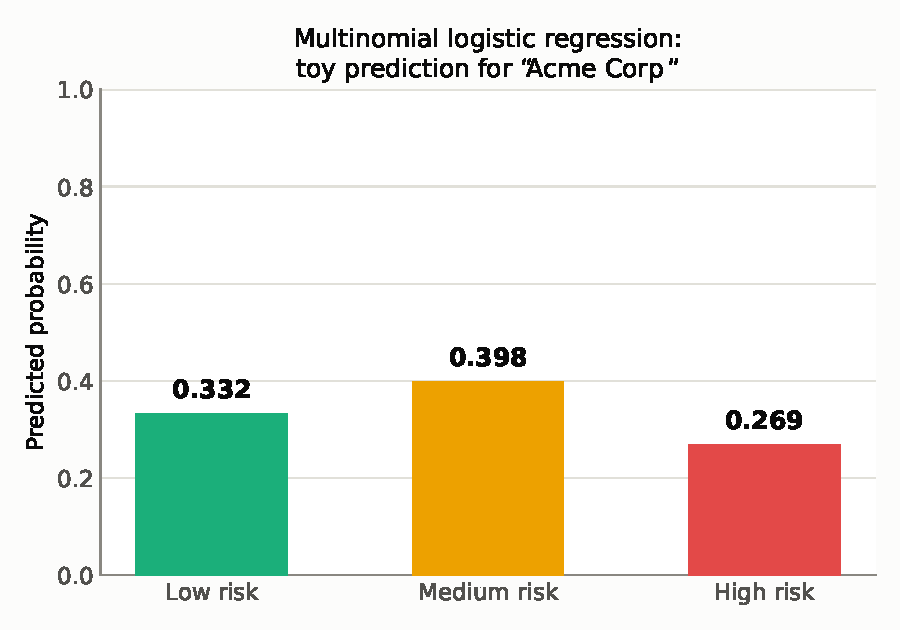
\includegraphics[width=\textwidth]{fig_softmax_bar.pdf}
      \end{figure}
    \end{column}
    \begin{column}{0.50\textwidth}
      \textbf{Applying the same formula to all 5 toy companies:}
      \renewcommand{\arraystretch}{1.15}
      \begin{center}
      \begin{tabular}{lccc}
        \toprule
        \textbf{Company} & $\Prob(\text{Low})$ & $\Prob(\text{Med})$ & $\Prob(\text{High})$\\
        \midrule
        Acme Corp   & 0.332 & \textbf{0.398} & 0.269\\
        Bolt Ind.   & 0.006 & 0.050 & \textbf{0.944}\\
        Cinder Ltd  & \textbf{0.860} & 0.131 & 0.009\\
        Delta Fr.   & \textbf{0.469} & 0.340 & 0.191\\
        Echo Sys.   & \textbf{0.807} & 0.165 & 0.028\\
        \bottomrule
      \end{tabular}
      \end{center}
      \vspace{0.3em}
      {\footnotesize Bold = predicted class (largest probability). Every row
      sums to 1.0, exactly as the softmax construction guarantees.}
    \end{column}
  \end{columns}
\end{frame}

% ── 6.2.2 ──────────────────────────────────────────────────────────────────────
\begin{frame}{6.2.2 Sparse Gaussian Processes -- Intuition}
  \begin{block}{Recap: what is a Gaussian process?}
    A \textbf{Gaussian process (GP)} is a non-parametric, probabilistic model:
    a prior over \emph{functions}, fully specified by a mean function
    $\mu(\x')$ and a kernel (covariance) function $k(\x_i',\x_j')$. Unlike a
    deep neural network, a GP naturally produces \textbf{uncertainty} around
    every prediction, not just a point estimate.
  \end{block}
  \begin{alertblock}{The scaling problem}
    Fitting an exact GP requires \textbf{inverting an $n\times n$ matrix}
    built from all $n$ training points --- an $O(n^3)$ operation. With
    thousands of companies and dozens of financial ratios, this quickly
    becomes infeasible.
  \end{alertblock}
  \textbf{Sparse GP idea:} instead of using all $n$ training points, summarize
  the dataset with a much smaller set of $m \ll n$ \textbf{inducing points}
  (pseudo-training examples). The number of inducing points is a user-chosen
  dial that trades off approximation quality against memory and compute cost.
\end{frame}

\begin{frame}{6.2.2 GP Regression: Mean and Variance (Eqs.\ 6.1--6.2)}
  \begin{block}{Setup (as in the book)}
    Training data $\{\x_t', \x_t\}_{t=1}^t$ with noisy observations
    $\x_t = f(\x_t') + \epsilon$, $\epsilon \sim \Norm(0,\sigma_X^2)$. The GP
    prior on $f$ is $f(\x') \sim \Norm(\mu_{x'}, \mathbf{K}_{x'} + \sigma_X^2\mathbf{I})$.
  \end{block}
  \begin{block}{Posterior predictive mean and variance at test point $\x_*'$}
    \[
      \Exp(f_*) = \mu_{\x_*'} + \mathbf{k}_* (K_{x'} + \sigma_X^2 \mathbf{I})^{-1}(\X - \mu_{x'})
      \tag{6.1}
    \]
    \[
      \mathrm{var}(f_*) = k_{**} - \mathbf{k}_*^\top (K_{x'} + \sigma_X^2 \mathbf{I})^{-1}\mathbf{k}_*
      \tag{6.2}
    \]
  \end{block}
  \textbf{Symbol guide:} $k_{**} = k(\x_*', \x_*')$ is the prior variance at
  the test point; $\mathbf{k}_* = k(\x', \x_*')$ is the vector of covariances
  between the training points and the test point; $\theta$ (kernel
  hyperparameters) and $\sigma_X$ (noise) are fit by maximizing the
  \textbf{log-marginal likelihood}
  $\log p(\X\mid\X') = \log \Norm\bigl(\mu_{x'}, \mathbf{K}_{x'x'}+\sigma_X^2\mathbf{I}\bigr)$ (Eq.\ 6.3).
\end{frame}

\begin{frame}{6.2.2 Making It Sparse: Inducing Points \& Variational Inference}
  \begin{itemize}
    \item \textbf{Inducing inputs} (pseudo-training examples) lower the rank
          of the matrix that must be inverted, cutting the cubic cost.
    \item Too few inducing points may miss local structure in fast-changing
          regions of the function; the user controls this trade-off.
    \item Sparse GPs generally \textbf{lack a closed-form solution}, so
          \textbf{variational inference} is used: Bayesian inference is
          recast as an optimization problem --- maximizing a \textbf{lower
          bound} on the log marginal likelihood.
    \item The locations of the pseudo-training points are treated as
          optimization arguments of the approximate posterior, learned
          \emph{jointly} with the model hyperparameters (likelihood and
          prior). This combination is the \textbf{sparse variational GP
          (SVGP)}.
  \end{itemize}
  \vspace{0.3em}
  \begin{alertblock}{Why this matters for credit ratings}
    With thousands of company-year observations across 26 financial and
    sector features, exact GPs are computationally out of reach --- SVGP
    with e.g.\ 100 or 500 inducing points keeps the model tractable.
  \end{alertblock}
\end{frame}

\begin{frame}[fragile]{Python: Sparse GP Predictive Mean/Variance (6.2.2)}
\begin{lstlisting}
import numpy as np

def sparse_gp_predict(Z, m_u, S_u, x_star, kernel, jitter=1e-6):
    """
    Toy sparse (variational) GP prediction using m inducing points.
    Z      : inducing input locations, shape (m, d)
    m_u    : variational mean at inducing points, shape (m,)
    S_u    : variational covariance at inducing points, shape (m, m)
    x_star : test input, shape (d,)
    kernel : covariance function k(x1, x2)
    """
    Kzz = np.array([[kernel(z_i, z_j) for z_j in Z] for z_i in Z])
    Kzz += jitter * np.eye(len(Z))
    Kzs = np.array([kernel(z_i, x_star) for z_i in Z])       # (m,)
    Kss = kernel(x_star, x_star)

    Kzz_inv = np.linalg.inv(Kzz)
    A = Kzz_inv @ Kzs                                          # (m,)

    mean = A @ m_u                                             # Eq. 6.1 analogue
    var  = Kss - Kzs @ Kzz_inv @ Kzs + A @ S_u @ A              # Eq. 6.2 analogue
    return mean, max(var, 0.0)

# In practice (e.g. GPflow), inducing locations Z, m_u, S_u, and kernel
# hyperparameters theta are all learned jointly by maximizing the ELBO
# (evidence lower bound on the log marginal likelihood).
\end{lstlisting}
\end{frame}

% ── 6.2.3 ──────────────────────────────────────────────────────────────────────
\begin{frame}{6.2.3 Distributed Gaussian Processes -- Intuition}
  \begin{block}{Plain-language idea}
    Instead of shrinking the data (as sparse GPs do), \textbf{distributed
    GPs} split a huge dataset into chunks, train a separate, smaller GP
    ``expert'' on each chunk, and then \textbf{combine} their predictions ---
    like asking several specialists for their opinion and pooling the
    answers. This lets the whole system scale to big data, and training can
    be spread across different compute clusters.
  \end{block}
  \begin{itemize}
    \item Each of $M$ experts is trained on its own data subset
          $D^j = \{\x^j, y^j\}$.
    \item Crucially, all experts \textbf{share the same kernel
          hyperparameters} $\theta$ --- this automatically regularizes the
          population, since no single expert can overfit its local subset.
    \item Assuming conditional independence across experts given the data,
          the shared log marginal likelihood is (Eq.\ 6.4):
          \[
            \log p(y\mid X,\theta) = \sum_{j=1}^{J} \log p_j(y\mid x^j,\theta^j)
          \]
    \item This chapter compares four combination rules: \textbf{PoE},
          \textbf{gPoE}, \textbf{BCM}, \textbf{rBCM} -- all differ only in
          \emph{how} the experts' Gaussian predictions are recombined.
  \end{itemize}
\end{frame}

\begin{frame}{6.2.3 Generalized Product of Experts (gPoE)}
  \begin{block}{Combining $M$ expert predictions at test point $x_*$ (Eq.\ 6.5)}
    \[
      p(f_* \mid x_*) \;\propto\; \prod_{j=1}^{J} p_j^{\,\beta_j(x_*)}(f_*\mid x_*, D^j)
    \]
  \end{block}
  \begin{block}{Predictive mean and precision (Eqs.\ 6.6--6.7)}
    \[
      m_{(g)poe}(x_*) = \sigma^2_{(g)poe}(x_*)\sum_{j=1}^{J}\beta_j(x_*)\,\sigma_j^{-2}(x_*)\,m_j(x_*)
    \]
    \[
      \sigma^{-2}_{(g)poe}(x_*) = \sum_{j=1}^{J}\beta_j(x_*)\,\sigma_j^{-2}(x_*)
    \]
  \end{block}
  \textbf{Symbol guide:} $D^j = \{x^j, y^j\}$ is the data given to expert
  $j$; $\beta_j(x_*)$ weights expert $j$'s contribution at $x_*$ (typically
  reflecting how confident that expert is there); setting $\beta_j(x_*)=1$
  for all $j$ recovers the plain \textbf{Product of Experts (PoE)}. As the
  number of experts grows, the product's aggregated variance can vanish,
  giving \textbf{overconfident} predictions -- a key weakness of PoE/gPoE.
\end{frame}

\begin{frame}{6.2.3 Robust Bayesian Committee Machine (rBCM)}
  \footnotesize
  \begin{block}{Predictive distribution via repeated Bayes' rule (Eq.\ 6.8)}
    Assuming conditional independence $D_i \perp\!\!\!\perp D_j \mid f_*$:
    \[
      p(f_*\mid x_*) = \frac{\displaystyle\prod_{j=1}^{J} p_j^{\,\beta_j(x_*)}(f_*\mid x_*, D^j)}
                             {\displaystyle p_j^{\,-1+\sum_{j=1}^{J}\beta_j(x_*)}(f_*\mid x_*)}
    \]
  \end{block}
  \vspace{-0.3em}
  \begin{block}{Predictive mean and precision (Eqs.\ 6.9--6.10)}
    \[
      m_{(r)bcm}(x_*) = \sigma^2_{(r)bcm}(x_*)\sum_{j=1}^{J}\beta_j(x_*)\,\sigma_j^{-2}(x_*)\,m_j(x_*)
    \]
    \[
      \sigma^{-2}_{(r)bcm}(x_*) = \sum_{j=1}^{J}\beta_j(x_*)\bigl(\sigma_j^{-2}(x_*)+\sigma_*^{-2}\bigr) + \sigma_*^{-2}
    \]
  \end{block}
  \vspace{-0.2em}
  Setting $\beta_j(x_*)=1$ for all $j$ recovers the plain \textbf{Bayesian
  Committee Machine (BCM)}. The extra prior-precision term $\sigma_*^{-2}$ is
  what guarantees the rBCM/BCM predictive distribution \textbf{reverts to the
  GP prior} away from the training data, unlike PoE/gPoE. This chapter
  considers all four: PoE, gPoE, BCM, rBCM.
\end{frame}

\begin{frame}{Toy Worked Example: Combining Two Gaussian Experts}
  \begin{block}{Setup: two toy expert predictions at the same test point}
    Expert 1: $\Norm(m_1, \sigma_1^2) = \Norm(2.0,\, 1.00)$ \quad(precision $\sigma_1^{-2}=1.00$)\\
    Expert 2: $\Norm(m_2, \sigma_2^2) = \Norm(3.0,\, 0.25)$ \quad(precision $\sigma_2^{-2}=4.00$)
  \end{block}
  \textbf{Step 1 -- combine precisions} (PoE special case, $\beta_j=1$ for all $j$):
  \[
    \sigma^{-2}_{poe} = \sigma_1^{-2} + \sigma_2^{-2} = 1.00 + 4.00 = 5.00
    \;\Longrightarrow\; \sigma^2_{poe} = \frac{1}{5.00} = 0.20
  \]
  \textbf{Step 2 -- combine means}, precision-weighted:
  \[
    m_{poe} = \sigma^2_{poe}\bigl(\sigma_1^{-2} m_1 + \sigma_2^{-2} m_2\bigr)
            = 0.20\times\bigl(1.00\times 2.0 + 4.00\times 3.0\bigr)
            = 0.20 \times 14.0 = 2.80
  \]
  \textbf{Result:} the combined (product-of-experts) prediction is
  $\Norm(2.80,\, 0.20)$ --- notice the combined variance (0.20) is
  \emph{smaller} than either expert's variance, and the combined mean
  (2.80) sits closer to Expert 2's mean because Expert 2 is more confident
  (smaller variance $\Rightarrow$ higher precision $\Rightarrow$ more
  ``weight'' in the average).
\end{frame}

\begin{frame}{Toy Illustration: Distributed GP on 1D Data}
  \begin{figure}
    \centering
    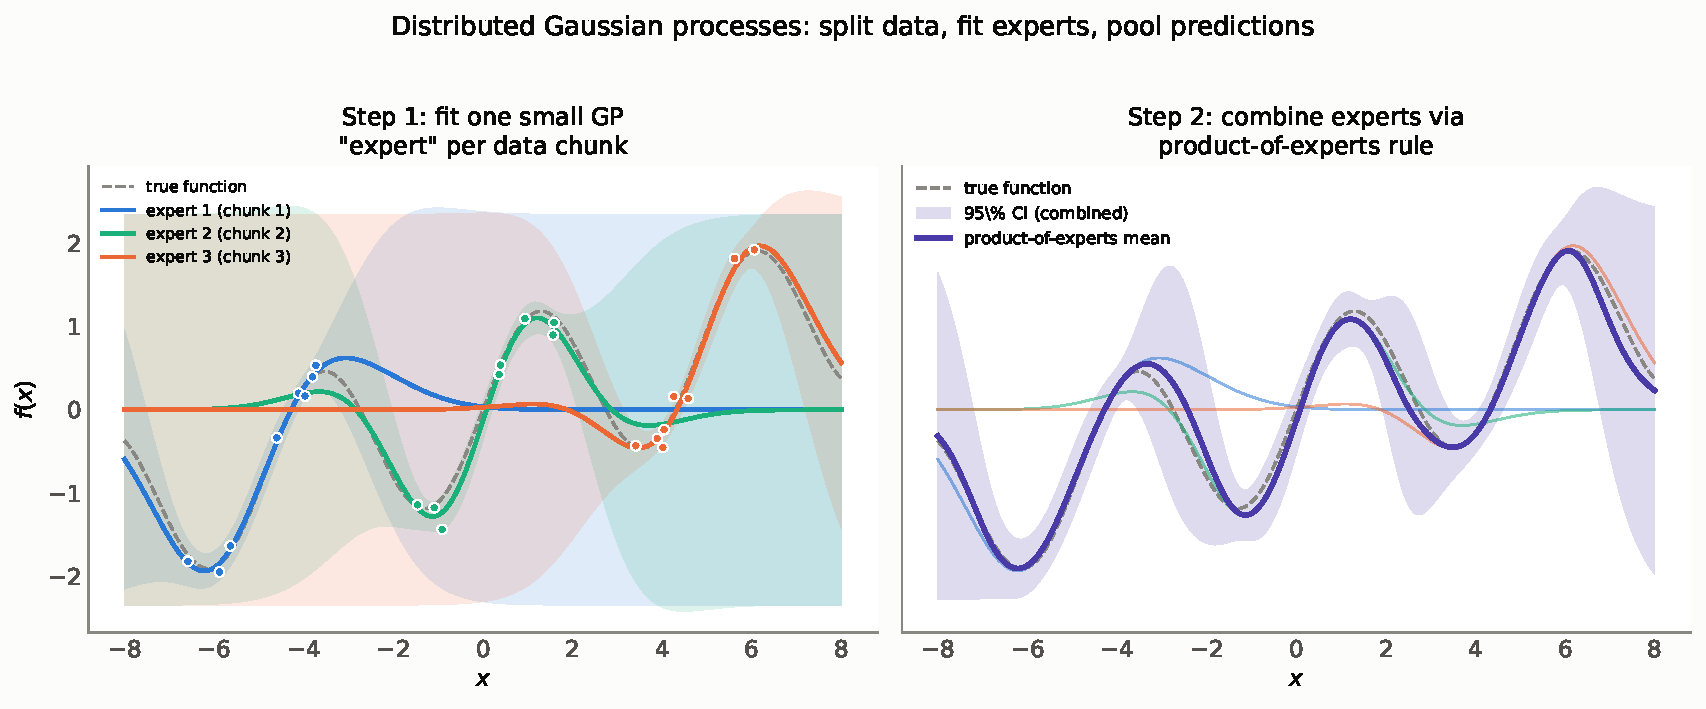
\includegraphics[width=0.92\textwidth]{fig_distributed_gp.pdf}
  \end{figure}
  \small A toy dataset is split into 3 chunks; a small GP expert is fitted
  to each chunk (left); the experts' Gaussian predictions are then combined
  via the product-of-experts rule into a single aggregated prediction
  (right, violet). This is the regression analogue of what happens (with a
  categorical likelihood layered on top) for the credit-rating
  \emph{classification} task in this chapter.
\end{frame}

\begin{frame}{Toy Illustration: From $M$ Experts to One Prediction}
  \begin{figure}
    \centering
    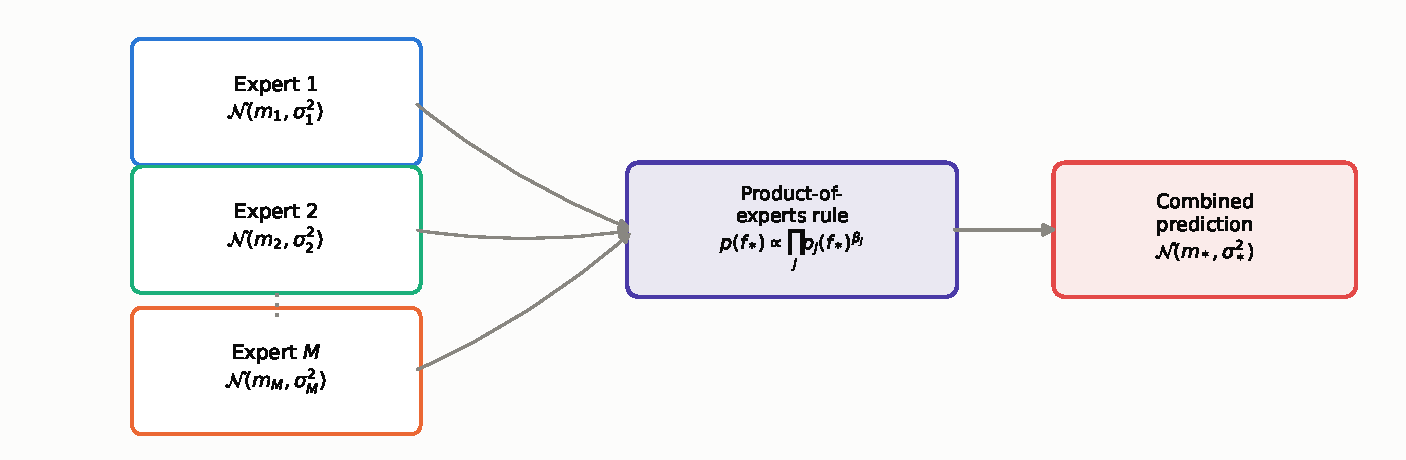
\includegraphics[width=0.95\textwidth]{fig_poe_flow.pdf}
  \end{figure}
  \centering \small Schematic flow: $M$ local GP experts, each producing its
  own Gaussian predictive distribution, are pooled via the product-of-experts
  rule into one combined Gaussian -- the mechanism underlying PoE, gPoE, BCM,
  and rBCM (they differ only in the weights $\beta_j(x_*)$ and the extra
  prior-precision term).
\end{frame}

\begin{frame}[fragile]{Python: Product-of-Experts Combination (6.2.3)}
\begin{lstlisting}
import numpy as np

def combine_experts(means, variances, betas=None):
    """
    Generalized product-of-experts combination (Eqs. 6.6-6.7).
    means, variances : arrays of shape (M,) -- one (m_j, sigma_j^2) per expert
    betas : per-expert confidence weights; betas=1 for all j -> plain PoE
    """
    M = len(means)
    if betas is None:
        betas = np.ones(M)                     # plain PoE (Eq. 6.7 with beta_j=1)

    precisions = 1.0 / np.asarray(variances)
    combined_precision = np.sum(betas * precisions)          # Eq. 6.7
    combined_variance  = 1.0 / combined_precision
    combined_mean = combined_variance * np.sum(
        betas * precisions * np.asarray(means))              # Eq. 6.6

    return combined_mean, combined_variance

# Toy two-expert example from the slides
m, v = combine_experts(means=[2.0, 3.0], variances=[1.00, 0.25])
print(m, v)   # -> 2.80  0.20
\end{lstlisting}
\end{frame}

% ══════════════════════════════════════════════════════════════════════════════
\section{6.3 Numerical Experiments}
% ══════════════════════════════════════════════════════════════════════════════

\begin{frame}[allowframebreaks]{6.3.1 Data Description}
  \begin{block}{The real dataset used in the book (not the toy example)}
    2021 credit rating observations on US corporations from the \textbf{three
    major international rating agencies}, each described by \textbf{26
    features}: 25 financial indicators plus the company's sector.
  \end{block}
  \textbf{The 25 financial indicators fall into five groups:}
  \begin{itemize}
    \item \textbf{Liquidity:} currentRatio, quickRatio, cashRatio,
          daysOfSalesOutstanding
    \item \textbf{Profitability:} grossProfitMargin, operatingProfitMargin,
          pretaxProfitMargin, netProfitMargin, effectiveTaxRate,
          returnOnAssets, returnOnEquity, returnOnCapitalEmployed
    \item \textbf{Debt:} debtRatio, debtEquityRatio
    \item \textbf{Operating performance:} assetTurnover
    \item \textbf{Cash flow:} operatingCashFlowPerShare, freeCashFlowPerShare,
          cashPerShare, operatingCashFlowSalesRatio,
          freeCashFlowOperatingCashFlowRatio
  \end{itemize}

  \framebreak

  \begin{block}{Target variable: mapping agency ratings to risk categories}
    \centering
    \renewcommand{\arraystretch}{1.1}
    \begin{tabular}{ll}
      \toprule
      \textbf{Credit rating(s)} & \textbf{Risk category}\\
      \midrule
      AAA & Lowest Risk (excluded -- too few observations)\\
      AA, A & Low Risk\\
      BBB & Medium Risk\\
      BB, B & High Risk\\
      CCC, CC, C & Highest Risk\\
      D & In Default (excluded)\\
      \bottomrule
    \end{tabular}
  \end{block}
  \vspace{0.3em}
  Entities in default (D) and the very-low-risk AAA band are excluded from
  the analysis, as both groups had too few observations.
\end{frame}

\begin{frame}{6.3.1 Class Distribution \& Pre-processing}
  \begin{columns}[T]
    \begin{column}{0.5\textwidth}
      \textbf{Distribution of risk categories} (as reported in the book):
      \begin{itemize}
        \item High Risk: 39\%
        \item Medium Risk: 33\%
        \item Low Risk: 24\%
        \item Highest Risk: 4\%
      \end{itemize}
      \vspace{0.3em}
      The classes are noticeably \textbf{imbalanced}, with the ``Highest
      Risk'' bucket being rare.
    \end{column}
    \begin{column}{0.46\textwidth}
      \textbf{Pre-processing:}
      \begin{itemize}
        \item 70/30 train--test split
        \item Features normalized with a \textbf{min--max scaler}
        \item All models share the same ARD squared-exponential kernel
              structure (where a kernel is used)
      \end{itemize}
    \end{column}
  \end{columns}
\end{frame}

\begin{frame}{6.3.2 Performance Metrics \& Experimental Settings}
  \begin{block}{Metrics on held-out (unseen) test data}
    \textbf{Accuracy}, \textbf{recall}, \textbf{precision}, and
    \textbf{F1-score} -- higher is better for all four.
  \end{block}
  \textbf{Models compared:}
  \begin{itemize}
    \item \textbf{MLR} -- the multinomial logistic regression benchmark
          (\S6.2.1).
    \item \textbf{SVGP} -- sparse variational GP, with \textbf{100} or
          \textbf{500} inducing points.
    \item \textbf{Distributed GPs} -- PoE, gPoE, BCM, rBCM, each with
          \textbf{100} or \textbf{200} experts (all using 100 inducing
          points per expert).
  \end{itemize}
  \vspace{0.2em}
  All GP variants use a \textbf{squared exponential kernel} with
  \textbf{automatic relevance determination (ARD)}, which lets the chapter
  extract a feature-importance ranking as a byproduct of training.
\end{frame}

% ══════════════════════════════════════════════════════════════════════════════
\section{6.4 Results and Discussions}
% ══════════════════════════════════════════════════════════════════════════════

\begin{frame}{6.4 Results: 100 Inducing Points / 100 Experts (Table 6.3)}
  \begin{center}
  \renewcommand{\arraystretch}{1.15}
  \footnotesize
  \begin{tabular}{lcccccc}
    \toprule
    \textbf{Metric} & MLR & SVGP$_{100}$ & PoE$_{100}$ & gPoE$_{100}$ & BCM$_{100}$ & rBCM$_{100}$\\
    \midrule
    Accuracy  & 0.384 & 0.542 & \textbf{0.611} & 0.606 & 0.601 & 0.606\\
    Recall    & 0.384 & 0.542 & \textbf{0.611} & 0.606 & 0.601 & 0.606\\
    Precision & 0.378 & 0.534 & \textbf{0.601} & 0.596 & 0.591 & 0.596\\
    F1        & 0.309 & 0.538 & \textbf{0.605} & 0.600 & 0.594 & 0.600\\
    \bottomrule
  \end{tabular}
  \end{center}
  \vspace{0.4em}
  \textbf{Key finding:} \textbf{PoE} outperforms across every metric in this
  setting; \textbf{MLR} is the weakest model; every distributed GP variant
  beats the SVGP model, which in turn beats MLR.
\end{frame}

\begin{frame}{6.4 Results: 500 Inducing Points / 200 Experts (Table 6.4)}
  \begin{center}
  \renewcommand{\arraystretch}{1.15}
  \footnotesize
  \begin{tabular}{lcccccc}
    \toprule
    \textbf{Metric} & MLR & SVGP$_{500}$ & PoE$_{200}$ & gPoE$_{200}$ & BCM$_{200}$ & rBCM$_{200}$\\
    \midrule
    Accuracy  & 0.384 & \textbf{0.571} & 0.532 & 0.532 & 0.532 & 0.532\\
    Recall    & 0.384 & \textbf{0.571} & 0.532 & 0.532 & 0.532 & 0.532\\
    Precision & 0.378 & \textbf{0.563} & 0.516 & 0.516 & 0.516 & 0.516\\
    F1        & 0.309 & \textbf{0.566} & 0.517 & 0.517 & 0.517 & 0.517\\
    \bottomrule
  \end{tabular}
  \end{center}
  \vspace{0.4em}
  \textbf{Key finding:} increasing the number of \textbf{inducing points}
  (100$\to$500) \textbf{improves} SVGP performance as expected -- but at a
  substantial increase in execution time. Increasing the number of
  \textbf{experts} (100$\to$200) instead \textbf{degrades} distributed GP
  performance. Choosing the right number of experts remains an open research
  problem.
\end{frame}

\begin{frame}{6.4 Which Features Matter Most? (Table 6.5, Figs.\ 6.2--6.3)}
  \begin{block}{Feature importance via ARD kernel length-scales}
    For every model, the \textbf{reciprocal of each feature's kernel
    length-scale} gives a natural importance score: the smaller the
    length-scale, the more sensitive predictions are to that feature, and
    the more important it is judged to be.
  \end{block}
  \renewcommand{\arraystretch}{1.05}
  \tiny
  \begin{center}
  \begin{tabular}{lllll}
    \toprule
    \textbf{Rank} & SVGP$_{100}$ & SVGP$_{500}$ & Distr.GP$_{100}$ & Distr.GP$_{200}$\\
    \midrule
    1 & operatingCashFlowSalesRatio & returnOnAssets & ebitPerRevenue & returnOnCapitalEmployed\\
    2 & returnOnCapitalEmployed & operatingCashFlowSalesRatio & operatingCashFlowSalesRatio & operatingCashFlowSalesRatio\\
    3 & debtRatio & returnOnCapitalEmployed & returnOnCapitalEmployed & netProfitMargin\\
    4 & grossProfitMargin & grossProfitMargin & pretaxProfitMargin & debtRatio\\
    5 & returnOnAssets & debtRatio & debtRatio & ebitPerRevenue\\
    \bottomrule
  \end{tabular}
  \end{center}
  \normalsize
  \vspace{0.3em}
  \textbf{Consensus:} all models broadly agree; \textbf{debtRatio},
  \textbf{operatingCashFlowSalesRatio}, and profit-margin-related metrics
  are consistently in the top 5.
\end{frame}

\begin{frame}{6.4 Discussion: Why These Features?}
  \begin{itemize}
    \item Firms with \textbf{high operatingCashFlowSalesRatio} and strong
          \textbf{profit margins} generate more cash relative to sales, so
          they are less likely to default -- intuitively, this pushes their
          rating \emph{up} (lower risk).
    \item Firms with \textbf{high debt ratios} are more heavily indebted,
          which impairs their ability to repay obligations -- this pushes
          their rating \emph{down} (higher risk).
    \item These results make intuitive financial sense and could be useful
          to stakeholders (lenders, regulators, investors) who want to
          understand \emph{what drives} a company's rating, not just the
          rating itself.
  \end{itemize}
  \vspace{0.3em}
  \begin{alertblock}{Overall summary of \S6.4}
    Distributed GPs $>$ sparse GP (SVGP) $>$ MLR benchmark, across almost
    every metric and setting -- but distributed GP performance
    \textbf{degrades} as the number of experts grows, an open modeling
    trade-off.
  \end{alertblock}
\end{frame}

% ══════════════════════════════════════════════════════════════════════════════
\section{6.5 Conclusion}
% ══════════════════════════════════════════════════════════════════════════════

\begin{frame}{6.5 Conclusion}
  \begin{block}{Summary}
    This chapter presented a first-in-literature Bayesian analysis of US
    corporate credit ratings using \textbf{sparse} and \textbf{distributed}
    Gaussian processes, benchmarked against \textbf{multinomial logistic
    regression}.
  \end{block}
  \begin{itemize}
    \item Distributed GPs (PoE, gPoE, BCM, rBCM) outperform both the sparse
          GP and the MLR benchmark across all performance metrics.
    \item Performance of distributed GPs \textbf{degenerates} as more
          experts are used -- the right number of experts is data- and
          task-dependent.
    \item The ARD kernel yields feature importances as a useful byproduct:
          \textbf{debt ratio}, \textbf{profit-margin} metrics, and
          \textbf{return-on-capital} metrics matter most for US corporate
          ratings.
  \end{itemize}
  \textbf{Future extensions noted by the authors:} try a \emph{mixture} of
  experts instead of a product of experts; apply the framework to data from
  a developing nation (e.g.\ South Africa); study principled ways to choose
  the number of experts.
  \vspace{0.2em}\\
  \textbf{Looking ahead:} Chapter 7 applies Hamiltonian Monte Carlo to model
  \emph{recovery rates} on charged-off loans -- another setting where
  understanding a portfolio's risk profile matters for lending decisions.
\end{frame}

% ══════════════════════════════════════════════════════════════════════════════
\begin{frame}[allowframebreaks]{Key Takeaways}
  \begin{block}{Multinomial logistic regression (\S6.2.1)}
    \begin{itemize}
      \item Multi-class generalization of logistic regression via the
            \textbf{softmax} link function.
      \item Each class gets a probability; all class probabilities sum to 1.
      \item Serves as the (weaker) benchmark model in this chapter.
    \end{itemize}
  \end{block}
  \begin{block}{Sparse Gaussian processes (\S6.2.2)}
    \begin{itemize}
      \item Exact GPs cost $O(n^3)$ -- infeasible at scale.
      \item Sparse GPs summarize the data with $m \ll n$ inducing points.
      \item Trained via variational inference (maximize a lower bound on the
            log marginal likelihood).
    \end{itemize}
  \end{block}
  \begin{block}{Distributed Gaussian processes (\S6.2.3)}
    \begin{itemize}
      \item Split data across $M$ experts, sharing kernel hyperparameters.
      \item Combine expert predictions via PoE, gPoE, BCM, or rBCM.
      \item PoE/gPoE can be overconfident as $M$ grows; BCM/rBCM correct
            this by reverting to the prior away from the data.
    \end{itemize}
  \end{block}

  \framebreak

  \begin{block}{Data and experiments (\S6.3)}
    \begin{itemize}
      \item 2021 credit rating observations, US corporations, 26 features
            (25 financial ratios + sector), mapped to 4 risk categories.
      \item 70/30 split, min--max scaled, evaluated via accuracy, recall,
            precision, F1.
    \end{itemize}
  \end{block}
  \begin{block}{Results (\S6.4)}
    \begin{itemize}
      \item Distributed GPs $>$ SVGP $>$ MLR across almost all settings.
      \item More inducing points help SVGP; more experts hurt distributed
            GPs.
      \item Debt ratio, cash-flow, and profit-margin ratios are the most
            important predictors across all models.
    \end{itemize}
  \end{block}
\end{frame}

\begin{frame}{Further Reading}
  \begin{columns}[T]
    \begin{column}{0.55\textwidth}
      \textbf{Key references (this chapter):}
      \begin{itemize}
        \item Cohen, Mbuvha, Marwala \& Deisenroth (2020). \emph{Healing
              products of Gaussian process experts}. ICML.
        \item Leibfried, Dutordoir, John \& Durrande (2020). \emph{A tutorial
              on sparse Gaussian processes and variational inference}.
              arXiv:2012.13962.
        \item Rasmussen \& Williams (2006). \emph{Gaussian Processes for
              Machine Learning}. MIT Press.
        \item Wallis, Kumar \& Gepp (2019). \emph{Credit rating forecasting
              using machine learning techniques}.
      \end{itemize}
    \end{column}
    \begin{column}{0.42\textwidth}
      \textbf{Next chapter:}\\
      Chapter 7 -- Hamiltonian Monte Carlo methods for modeling recovery
      rates on charged-off loans.
      \vspace{0.5em}
      \begin{itemize}
        \item Portfolio-level lending decisions
        \item Advanced HMC sampling
        \item Continuing the Bayesian ML theme in credit risk
      \end{itemize}
    \end{column}
  \end{columns}
\end{frame}

\end{document}
